\documentclass[fleqn,10pt]{wlscirep}
\usepackage[utf8]{inputenc}
\usepackage[T1]{fontenc}
\usepackage{pgfplots}
\usepackage{pgfplotstable}
\pgfplotsset{compat=1.18}
\usepackage{booktabs}
\usepackage{multirow}
\usepackage{amsmath}
\usepackage{filecontents}
\usepackage{xcolor}
\usepackage{colortbl}
\usepackage{array}
\usepackage{url}
\usepackage{tikz}
\usetikzlibrary{shapes.geometric, arrows.meta, positioning, fit, calc}

% ============================================================
% Inline data files for pgfplots
% ============================================================

\begin{filecontents*}{content_engagement.csv}
Type,N,VisPct,VisScore,TrPct,TrScore
HandsOn,2189,64.1,58.9,12.5,10.7
Diagram,1882,52.1,48.0,22.2,19.2
Animation,385,50.3,46.4,21.2,18.2
EquipClose,1033,48.9,44.8,15.7,13.7
Presenter,1545,47.6,44.0,21.8,19.1
Slides,1265,47.1,43.1,22.8,20.1
Device,447,39.2,36.6,20.4,18.2
Screen,1144,35.6,32.7,13.1,11.3
Other,107,31.2,29.4,13.4,12.0
\end{filecontents*}

\begin{filecontents*}{content_dist_conv.csv}
Type,Pct
HandsOn,6.4
EquipClose,8.3
Presenter,21.2
Slides,17.6
Diagram,29.6
Screen,8.3
Animation,5.6
Device,2.3
Other,0.7
\end{filecontents*}

\begin{filecontents*}{content_dist_verb.csv}
Type,Pct
HandsOn,27.0
EquipClose,11.1
Presenter,12.9
Slides,9.8
Diagram,11.0
Screen,17.6
Animation,2.4
Device,6.9
Other,1.3
\end{filecontents*}

\begin{filecontents*}{content_dist_vis.csv}
Type,Pct
HandsOn,70.0
EquipClose,16.3
Presenter,0.0
Slides,1.5
Diagram,0.4
Screen,3.3
Animation,1.3
Device,5.4
Other,1.8
\end{filecontents*}

\begin{filecontents*}{hands_by_subgroup.csv}
Label,VisPct
Conv,43.9
VerbEmb,67.1
VisEmb,67.8
\end{filecontents*}

\begin{filecontents*}{density_data.csv}
Density,N,VisPct,VisScore
1,1169,45.2,41.6
2,1137,52.4,48.4
3,2562,48.4,44.5
4,3255,52.4,48.4
5,1874,51.1,46.9
\end{filecontents*}


% ============================================================
% Title and authors
% ============================================================
\title{Multimodal Fusion Analysis of Visual and Verbal Engagement in Embodied Robotics Instruction}

\author[1,*]{Hongbo Zhang}
\author[1]{Benjamin Li}
\author[1]{Reshma Rajan}
\author[1]{Natalie Galvan}
\affil[1]{Department of Engineering Technology, Middle Tennessee State University, Murfreesboro, TN 37132, USA}

\affil[*]{hbzhang@mtsu.edu}

\begin{abstract}
Prior research on embodied learning in robotics education has relied primarily on transcript-based metrics, which inherently undervalue instructional approaches that communicate through physical demonstration rather than verbal narration. This study introduces a multimodal fusion framework that jointly analyzes visual and verbal channels of engagement at the segment level, enabling a mechanistic understanding of how specific content types drive viewer interaction. We analyzed 130 robotics instructional videos (56 conventional, 48 verbally embodied, 26 visually embodied), segmenting each into 10-second intervals and classifying each segment by content type using Gemini 2.0 Flash video understanding. Visual and transcript correlation scores were computed by measuring semantic alignment between viewer comments and frame captions or transcripts for each segment. Our results demonstrate that hands-on demonstration segments achieve significantly higher visual engagement (64.1\% correlated) than slide-based (47.1\%) or screen-based (35.6\%) content ($F = 49.4$, $p < 10^{-79}$). A two-way ANOVA reveals that the subgroup main effect becomes non-significant ($p = 0.191$) after controlling for content type, indicating that content composition---not instructional label---drives the engagement difference. Multiple regression confirms that hands-on content ($\beta = +6.2$, $p < 0.001$) and hand visibility ($\beta = +3.6$, $p < 0.001$) are significant positive predictors, while screen content ($\beta = -13.2$, $p < 10^{-14}$) is the strongest negative predictor. At the video level, the proportion of hands-on content correlates strongly with visual engagement among verbally embodied videos ($r = 0.53$, $p < 10^{-4}$). Temporal analysis reveals that engagement declines over the course of a video in conventional instruction ($F = 9.5$, $p < 10^{-4}$) but remains sustained in visually embodied videos. These findings establish that the engagement advantage of embodied instruction is driven by the specific visual content it delivers---physical demonstrations, visible manipulation, and equipment interaction---rather than by the instructional modality per se, reversing the ranking obtained by transcript-only analysis.
\end{abstract}

\begin{document}

\flushbottom
\maketitle
\thispagestyle{empty}

% ============================================================
% INTRODUCTION
% ============================================================
\section*{Introduction}

Embodied learning theory posits that cognitive processes are fundamentally grounded in bodily experience, and that physical interaction with learning materials enhances comprehension, retention, and transfer~\cite{wilson2002six,barsalou2008grounded}. In robotics education, this principle manifests as hands-on instruction---hardware assembly, wiring, calibration, and real-time operation---in contrast to conventional lecture-based approaches that rely on slides, diagrams, and verbal explanation~\cite{johnson2014embodied}. While the theoretical advantages of embodied instruction are well established, empirical quantification of how visual and verbal modalities independently contribute to learner engagement remains limited.

Our prior work~\cite{zhang2025transcript} examined engagement in the same corpus of 130 robotics videos using transcript-based semantic correlation. That analysis revealed a confound: embodied videos appeared to underperform conventional videos on transcript metrics because a subset (26 of 74) were silent demonstrations with minimal narration. After isolating verbally narrated embodied videos, the transcript-based correlation gap narrowed substantially, demonstrating that skilled verbal narration of physical procedures can be as effective as conventional lecture delivery for generating topically aligned viewer responses.

However, transcript-only analysis cannot capture the visual dimension of engagement that is central to embodied instruction. When an instructor demonstrates soldering a circuit or calibrating a sensor, the visual content communicates instructional information that the transcript may not encode. Viewer comments responding to what they \emph{see} rather than what they \emph{hear} are invisible to transcript-based metrics. This creates a systematic bias against embodied instruction, whose pedagogical value is disproportionately carried by the visual channel.

To address this limitation, this study introduces a multimodal fusion framework that jointly analyzes visual and verbal engagement at the segment level. Each video is divided into 10-second segments, and viewer comments are correlated with both frame-level visual captions and transcript excerpts independently. This dual-channel approach enables us to measure how much of a viewer's response is driven by visual content versus verbal content, and to identify which specific content types---hands-on demonstrations, equipment close-ups, diagrams, slides, screen recordings---generate the highest engagement.

We further employ large multimodal model-based video classification to categorize each segment's content type, audio-visual alignment, and instructional features directly from the raw video. This segment-level classification enables a shift from group-level comparisons (embodied vs.\ conventional) to a mechanistic analysis of \emph{what} content features drive engagement and \emph{why} embodied videos achieve higher visual correlation scores.

Our central hypothesis is that the engagement advantage of embodied instruction is attributable to the specific visual content it delivers---physical demonstrations, visible hand manipulation, and equipment interaction---rather than to the instructional category label itself. If correct, then (1) content type should remain a significant predictor of engagement after controlling for subgroup, (2) the subgroup effect should diminish or vanish when content type is included as a covariate, and (3) the proportion of hands-on content within a video should predict its overall engagement at the video level.


% ============================================================
% RESULTS
% ============================================================
\section*{Results}

\subsection*{Segment-level engagement by content type}

To test whether specific visual content types drive viewer engagement, we computed the visual and transcript correlation scores for each of the nine content categories across all 9{,}997 classified segments. Figure~\ref{fig:vis_by_content} presents the percentage of segments that achieved a positive visual correlation (visual correlation score $> 0$) for each content type, ordered by visual engagement.

\begin{figure}[ht]
    \centering
    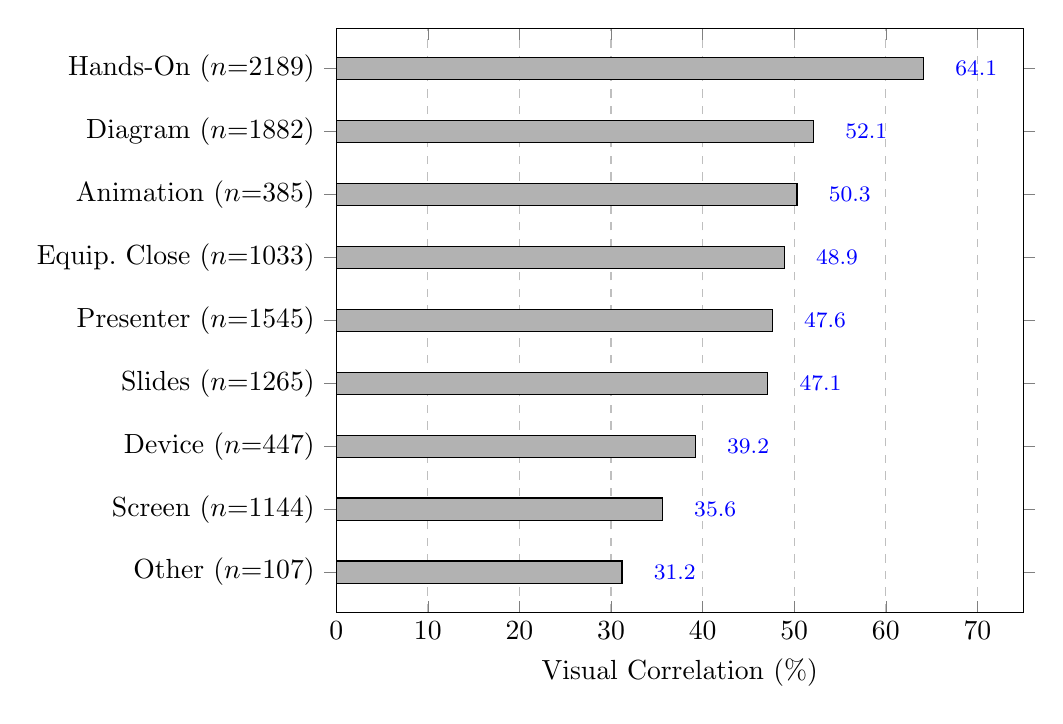
\begin{tikzpicture}
        \begin{axis}[
            xbar,
            bar width=8pt,
            width=0.85 \columnwidth,
            height=9cm,
            xlabel={Visual Correlation (\%)},
            xmin=0, xmax=75,
            symbolic y coords={Other,Screen,Device,Slides,Presenter,EquipClose,Animation,Diagram,HandsOn},
            ytick=data,
            yticklabels={Other ($n$=107),Screen ($n$=1144),Device ($n$=447),Slides ($n$=1265),Presenter ($n$=1545),Equip.\ Close ($n$=1033),Animation ($n$=385),Diagram ($n$=1882),Hands-On ($n$=2189)},
            nodes near coords,
            nodes near coords style={font=\footnotesize, xshift=8pt},
            xmajorgrids=true,
            grid style=dashed,
            enlarge y limits=0.08,
        ]
            \addplot+[fill=gray!60, draw=black] coordinates {
                (31.2,Other)
                (35.6,Screen)
                (39.2,Device)
                (47.1,Slides)
                (47.6,Presenter)
                (48.9,EquipClose)
                (50.3,Animation)
                (52.1,Diagram)
                (64.1,HandsOn)
            };
        \end{axis}
    \end{tikzpicture}
    \caption{Percentage of segments with positive visual correlation by content type. Hands-on demonstration segments achieve the highest visual engagement at 64.1\%, significantly exceeding all other categories.}
    \label{fig:vis_by_content}
\end{figure}

Hands-on demonstration segments achieve the highest visual engagement at 64.1\%, followed by diagram/whiteboard (52.1\%) and animation/graphic (50.3\%) content. Screen/software recordings show the lowest engagement among instructional content types at 35.6\%. A one-way ANOVA confirms that the differences across content types are highly significant ($F = 49.4$, $p < 10^{-79}$). Pairwise $t$-tests reveal that hands-on demonstrations significantly outperform slides ($t = 10.9$, $p < 10^{-27}$, Cohen's $d = 0.39$), presenter-talking segments ($t = 10.8$, $p < 10^{-26}$, $d = 0.39$), and diagram segments ($t = 8.7$, $p < 10^{-18}$).

Table~\ref{tab:engagement_by_content} provides the complete engagement metrics for each content type across both visual and transcript channels.

\begin{table}[ht]
    \centering
    \caption{Segment-level engagement metrics by content type. Vis.\ Corr.\ and Tr.\ Corr.\ denote the percentage of segments with positive visual and transcript correlation, respectively. Vis.\ Score and Tr.\ Score are the mean correlation scores (0--100).}
    \label{tab:engagement_by_content}
    \begin{tabular}{lrcccc}
        \toprule
        Content Type & $n$ & \multicolumn{2}{c}{Visual} & \multicolumn{2}{c}{Transcript} \\
        \cmidrule(lr){3-4} \cmidrule(lr){5-6}
        & & Corr.\% & Score & Corr.\% & Score \\
        \midrule
        Hands-on demo & 2189 & \textbf{64.1} & \textbf{58.9} & 12.5 & 10.7 \\
        Diagram/whiteboard & 1882 & 52.1 & 48.0 & 22.2 & 19.2 \\
        Animation/graphic & 385 & 50.3 & 46.4 & 21.2 & 18.2 \\
        Equipment closeup & 1033 & 48.9 & 44.8 & 15.7 & 13.7 \\
        Presenter talking & 1545 & 47.6 & 44.0 & 21.8 & 19.1 \\
        Slide/PowerPoint & 1265 & 47.1 & 43.1 & \textbf{22.8} & \textbf{20.1} \\
        Device in operation & 447 & 39.2 & 36.6 & 20.4 & 18.2 \\
        Screen/software & 1144 & 35.6 & 32.7 & 13.1 & 11.3 \\
        Other & 107 & 31.2 & 29.4 & 13.4 & 12.0 \\
        \bottomrule
    \end{tabular}
\end{table}

Notably, the transcript correlation pattern diverges from visual correlation: slide and diagram content show the highest transcript correlation (22.8\% and 22.2\%, respectively), while hands-on demonstrations rank lowest (12.5\%). This inverse relationship confirms that hands-on content drives engagement primarily through the visual channel, and that transcript-only analyses systematically underestimate its instructional impact.


\subsection*{Content distribution across subgroups}

Having established that content type significantly predicts engagement, we examined how content types are distributed across the three instructional subgroups. Figure~\ref{fig:content_dist} compares the proportion of hands-on demonstration content across subgroups.

\begin{figure}[ht]
    \centering
    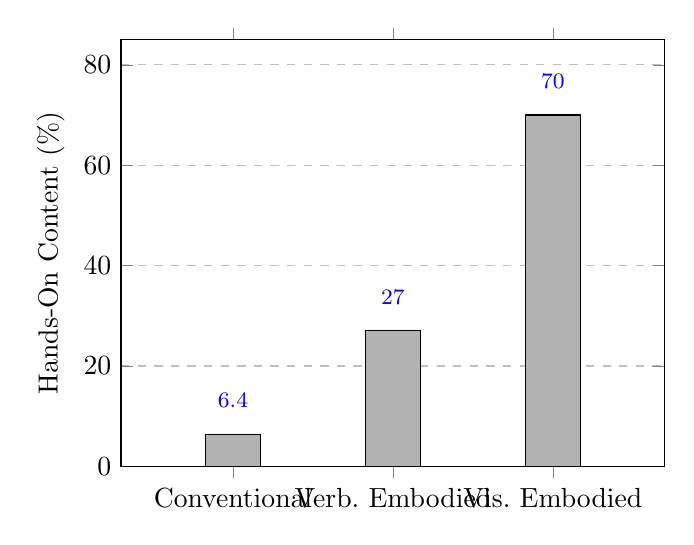
\begin{tikzpicture}
        \begin{axis}[
            ybar,
            bar width=20pt,
            width=0.7\linewidth,
            height=7cm,
            symbolic x coords={Conv,VerbEmb,VisEmb},
            xtick=data,
            xticklabels={Conventional,Verb.\ Embodied,Vis.\ Embodied},
            ylabel={Hands-On Content (\%)},
            ymin=0, ymax=85,
            enlarge x limits=0.35,
            nodes near coords,
            nodes near coords style={font=\bfseries\footnotesize, yshift=6pt},
            ymajorgrids=true,
            grid style=dashed,
        ]
            \addplot+[fill=gray!60, draw=black] coordinates {
                (Conv,6.4)
                (VerbEmb,27.0)
                (VisEmb,70.0)
            };
        \end{axis}
    \end{tikzpicture}
    \caption{Proportion of hands-on demonstration segments by subgroup. Visually embodied videos dedicate 70.0\% of their content to hands-on demonstration, compared to 27.0\% for verbally embodied and 6.4\% for conventional videos.}
    \label{fig:content_dist}
\end{figure}

The contrast is stark: visually embodied videos dedicate 70.0\% of their segments to hands-on demonstration, verbally embodied videos 27.0\%, and conventional videos only 6.4\%. Conversely, conventional videos are dominated by diagram/whiteboard (29.6\%), presenter-talking (21.2\%), and slide content (17.6\%). Table~\ref{tab:content_dist} presents the full content distribution for all three subgroups.

\begin{table}[ht]
    \centering
    \caption{Content type distribution (\%) by instructional subgroup. Dominant content types for each subgroup are shown in bold.}
    \label{tab:content_dist}
    \begin{tabular}{lccc}
        \toprule
        Content Type & Conv. & Verb.\ Emb. & Vis.\ Emb. \\
        \midrule
        Hands-on demo & 6.4 & \textbf{27.0} & \textbf{70.0} \\
        Equipment closeup & 8.3 & 11.1 & 16.3 \\
        Presenter talking & \textbf{21.2} & 12.9 & 0.0 \\
        Slide/PowerPoint & 17.6 & 9.8 & 1.5 \\
        Diagram/whiteboard & \textbf{29.6} & 11.0 & 0.4 \\
        Screen/software & 8.3 & 17.6 & 3.3 \\
        Animation/graphic & 5.6 & 2.4 & 1.3 \\
        Device in operation & 2.3 & 6.9 & 5.4 \\
        Other & 0.7 & 1.3 & 1.8 \\
        \bottomrule
    \end{tabular}
\end{table}

This distribution pattern provides the mechanistic link between instructional modality and engagement: embodied videos achieve higher visual engagement not because of an intrinsic quality of ``embodied instruction,'' but because they contain substantially more of the content type (hands-on demonstration) that generates the highest visual correlation.


\subsection*{Content type mediates the subgroup effect}

The previous analyses established two facts: (1) content type predicts engagement, and (2) subgroups differ in content composition. A critical question follows: does the subgroup label carry any independent explanatory power after content type is accounted for? To test this, we conducted a two-way ANOVA with content type and subgroup as factors, including their interaction.

Table~\ref{tab:twoway} presents the results. Content type remains a strong predictor ($F = 39.5$, $p < 10^{-54}$, $\eta^2 = 3.03\%$). However, the subgroup main effect---which was highly significant in the one-way ANOVA ($F = 99.4$, $p < 10^{-43}$)---becomes non-significant when content type is included ($F = 1.7$, $p = 0.191$, $\eta^2 = 0.03\%$). The interaction term is significant ($F = 8.4$, $p < 10^{-19}$, $\eta^2 = 1.29\%$), indicating that the same content type generates different engagement levels depending on the subgroup.

\begin{table}[ht]
    \centering
    \caption{Two-way ANOVA results for visual engagement score. The subgroup main effect becomes non-significant after controlling for content type, indicating full mediation.}
    \label{tab:twoway}
    \begin{tabular}{lrccc}
        \toprule
        Source & $F$ & $p$-value & $\eta^2$ (\%) \\
        \midrule
        Content type & 39.5 & $< 10^{-54}$ & 3.03 \\
        Subgroup & 1.7 & 0.191 & 0.03 \\
        Content type $\times$ Subgroup & 8.4 & $< 10^{-19}$ & 1.29 \\
        \bottomrule
    \end{tabular}
\end{table}

This result provides direct statistical evidence for the mediation hypothesis: the subgroup-level engagement advantage of embodied instruction is entirely attributable to the content types those videos employ. Once content type is controlled, knowing whether a video is ``conventional'' or ``embodied'' provides no additional information about its visual engagement. The significant interaction reflects the finding that embodied instructors produce higher-quality hands-on demonstrations (67.1--67.8\% visual correlation vs.\ 43.9\% for conventional hands-on content), as reported in the subgroup-level analysis below.


\subsection*{Subgroup-level visual engagement}

To quantify the subgroup-level engagement difference, we compared the overall visual correlation across the three subgroups. A one-way ANOVA reveals highly significant differences ($F = 99.4$, $p < 10^{-43}$). Figure~\ref{fig:subgroup_vis} presents the visual correlation percentage for hands-on demonstration segments specifically, broken down by subgroup.

\begin{figure}[ht]
    \centering
    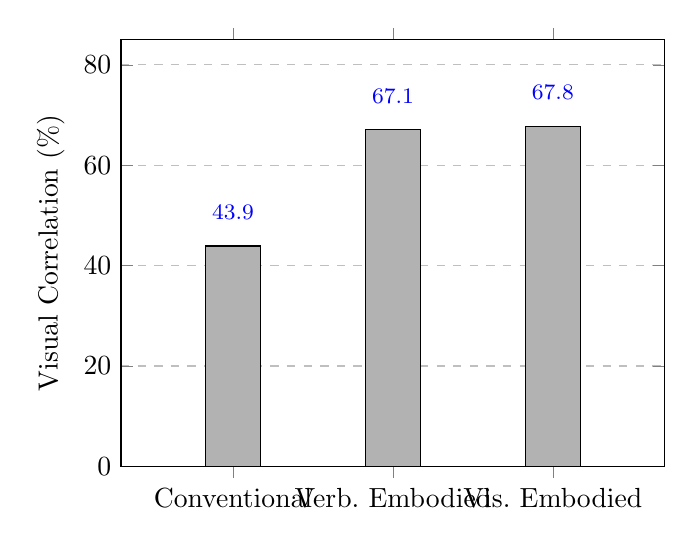
\begin{tikzpicture}
        \begin{axis}[
            ybar,
            bar width=20pt,
            width=0.7\linewidth,
            height=7cm,
            symbolic x coords={Conv,VerbEmb,VisEmb},
            xtick=data,
            xticklabels={Conventional,Verb.\ Embodied,Vis.\ Embodied},
            ylabel={Visual Correlation (\%)},
            ymin=0, ymax=85,
            enlarge x limits=0.35,
            nodes near coords,
            nodes near coords style={font=\bfseries\footnotesize, yshift=6pt},
            ymajorgrids=true,
            grid style=dashed,
        ]
            \addplot+[fill=gray!60, draw=black] coordinates {
                (Conv,43.9)
                (VerbEmb,67.1)
                (VisEmb,67.8)
            };
        \end{axis}
    \end{tikzpicture}
    \caption{Visual correlation of hands-on demonstration segments by subgroup. Embodied videos achieve substantially higher visual engagement for the same content type, suggesting that embodied instructors produce higher-quality hands-on demonstrations.}
    \label{fig:subgroup_vis}
\end{figure}

An important nuance emerges: even within the same content type (hands-on demonstration), embodied videos achieve substantially higher visual correlation (67.1\% verbally embodied, 67.8\% visually embodied) than conventional videos (43.9\%). This indicates that the engagement advantage of embodied instruction is twofold: (1) embodied videos contain more hands-on content, and (2) the hands-on content in embodied videos is itself more engaging---likely because embodied instructors are more skilled at producing compelling physical demonstrations. This within-content-type subgroup difference accounts for the significant interaction term in the two-way ANOVA.


\subsection*{Multiple regression analysis}

To estimate the relative contribution of each predictor while controlling for all others, we fit an ordinary least squares (OLS) regression model predicting visual engagement score from content type, hand visibility, narration, instructional density, and subgroup. Table~\ref{tab:regression} presents the model coefficients.

\begin{table}[ht]
    \centering
    \caption{OLS regression predicting visual engagement score. Reference categories: slide/PowerPoint (content type), conventional (subgroup). $R^2 = 0.050$, $F = 40.2$, $p < 10^{-100}$.}
    \label{tab:regression}
    \begin{tabular}{lrrrl}
        \toprule
        Predictor & $\beta$ & SE & $t$ & $p$ \\
        \midrule
        Intercept & 35.5 & 2.08 & 17.1 & $< 0.001$ \\
        \addlinespace
        \multicolumn{5}{l}{\textit{Content type (vs.\ slide/PowerPoint)}} \\
        \quad Hands-on demo & +6.2 & 1.84 & 3.4 & $< 0.001$ \\
        \quad Diagram/whiteboard & +3.9 & 1.53 & 2.6 & 0.010 \\
        \quad Animation/graphic & +3.6 & 2.37 & 1.5 & 0.128 \\
        \quad Equipment closeup & $-2.5$ & 1.86 & $-1.3$ & 0.186 \\
        \quad Presenter talking & $-0.9$ & 1.71 & $-0.5$ & 0.585 \\
        \quad Device in operation & $-10.1$ & 2.36 & $-4.3$ & $< 0.001$ \\
        \quad Screen/software & $-13.2$ & 1.70 & $-7.8$ & $< 10^{-14}$ \\
        \quad Other & $-13.7$ & 4.26 & $-3.2$ & 0.001 \\
        \addlinespace
        \multicolumn{5}{l}{\textit{Segment features}} \\
        \quad Hands visible & +3.6 & 1.09 & 3.3 & $< 0.001$ \\
        \quad Narration present & +3.1 & 1.72 & 1.8 & 0.069 \\
        \quad Instructional density & +0.7 & 0.41 & 1.6 & 0.106 \\
        \addlinespace
        \multicolumn{5}{l}{\textit{Subgroup (vs.\ conventional)}} \\
        \quad Verbally embodied & +6.0 & 0.96 & 6.2 & $< 10^{-9}$ \\
        \quad Visually embodied & +16.4 & 1.79 & 9.2 & $< 10^{-19}$ \\
        \bottomrule
    \end{tabular}
\end{table}

The model is highly significant ($F = 40.2$, $p < 10^{-100}$) with $R^2 = 0.050$. Among content types, hands-on demonstration ($\beta = +6.2$) and diagram/whiteboard ($\beta = +3.9$) are the only significant positive predictors relative to slides. Screen/software content is the strongest negative predictor ($\beta = -13.2$, $p < 10^{-14}$), followed by device-in-operation ($\beta = -10.1$). Hand visibility provides a significant independent contribution ($\beta = +3.6$, $p < 0.001$) after controlling for content type, confirming that the physical presence of hands adds engagement value beyond the content classification itself. Narration and instructional density do not reach significance ($p = 0.069$ and $p = 0.106$, respectively).

The subgroup coefficients remain significant in the regression ($\beta = +6.0$ for verbally embodied, $\beta = +16.4$ for visually embodied), consistent with the significant interaction in the two-way ANOVA: even after accounting for content type and segment features, embodied videos generate higher visual engagement, reflecting the quality advantage identified in the within-content-type analysis.

The modest $R^2$ of 0.050 reflects the high variance inherent in segment-level engagement data, where individual viewer comment--segment pairs introduce substantial noise. The model's significance and consistent coefficient signs indicate reliable directional effects despite this variance.


\subsection*{Video-level analysis}

To complement the segment-level analyses, we aggregated engagement metrics to the video level ($N = 128$ videos with complete data) and examined whether the proportion of hands-on content in a video predicts its overall visual engagement. Figure~\ref{fig:video_scatter} presents this relationship for verbally embodied videos, where the correlation is strongest.

\begin{figure}[ht]
    \centering
    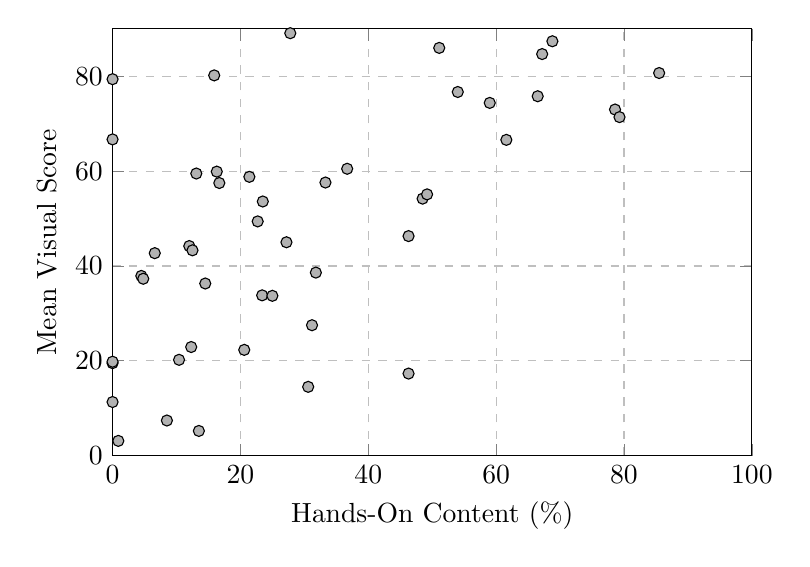
\begin{tikzpicture}
        \begin{axis}[
            width=0.8\linewidth,
            height=7cm,
            xlabel={Hands-On Content (\%)},
            ylabel={Mean Visual Score},
            xmin=0, xmax=100,
            ymin=0, ymax=90,
            grid=both,
            grid style=dashed,
            only marks,
            mark=*,
            mark size=2pt,
        ]
            % Verbally embodied videos (48 data points from video_level_metrics.csv)
            \addplot+[mark options={fill=gray!60, draw=black}] coordinates {
                (0.0,79.4) (0.0,19.5) (0.0,66.7) (0.0,11.3) (0.0,19.8)
                (0.9,3.1) (3.9,91.0) (4.5,37.9) (4.8,37.3) (6.6,42.7)
                (8.5,7.4) (10.4,20.2) (12.0,44.2) (12.3,22.9) (12.5,43.3)
                (13.1,59.5) (13.5,5.2) (14.5,36.3) (15.9,80.2) (16.3,59.9)
                (16.7,57.5) (20.6,22.3) (21.4,58.8) (22.7,49.4) (23.4,33.8)
                (23.5,53.6) (25.0,33.7) (27.2,45.0) (27.8,89.1) (30.6,14.5)
                (31.2,27.5) (31.8,38.6) (33.3,57.6) (36.7,60.5) (46.3,46.3)
                (46.3,17.3) (48.5,54.2) (49.2,55.1) (51.1,86.0) (54.0,76.7)
                (59.0,74.4) (61.6,66.6) (66.5,75.8) (67.2,84.7) (68.8,87.4)
                (78.6,73.0) (79.3,71.4) (85.5,80.7)
            };
            % Best fit line: y = 33.8 + 0.547x (OLS from actual data)
            \addplot[black, thick, domain=0:90, samples=2] {33.8 + 0.547*x};
        \end{axis}
    \end{tikzpicture}
    \caption{Video-level relationship between hands-on content proportion and mean visual engagement for verbally embodied videos ($n = 48$). Pearson $r = 0.53$, $p < 10^{-4}$. The fitted line illustrates the positive trend.}
    \label{fig:video_scatter}
\end{figure}

Among verbally embodied videos, the proportion of hands-on content shows a strong positive correlation with mean visual engagement ($r = 0.53$, $p = 1.2 \times 10^{-4}$, $n = 48$). This video-level result confirms that the segment-level content type effect scales up: videos that dedicate more time to physical demonstrations receive higher overall visual engagement from viewers.

The overall correlation across all 128 videos is $r = 0.33$ ($p = 1.2 \times 10^{-4}$). Within conventional videos, the correlation is negligible ($r = -0.03$, $p = 0.81$, $n = 55$), reflecting the fact that conventional videos contain very little hands-on content (mean 6.4\%), leaving insufficient variance to detect a relationship. Among visually embodied videos, the correlation is also weak ($r = 0.04$, $p = 0.85$, $n = 25$) because these videos are already saturated with hands-on content (mean 70.0\%), creating a ceiling effect.


\subsection*{Effect of visible hands}

Visibility of the instructor's hands during a segment provides a direct marker of physical interaction. Across all 9{,}997 segments, those with visible hands ($n = 4{,}978$) show significantly higher visual correlation (56.3\%) than those without ($n = 5{,}019$; 44.3\%), as shown in Figure~\ref{fig:hands_effect}. This 12.0 percentage-point difference is highly significant ($p < 10^{-40}$, Welch's $t$-test).

\begin{figure}[ht]
    \centering
    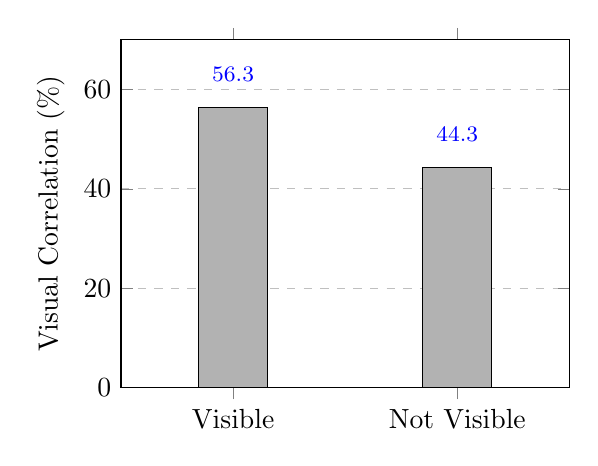
\begin{tikzpicture}
        \begin{axis}[
            ybar,
            bar width=25pt,
            width=0.6\linewidth,
            height=6cm,
            symbolic x coords={Visible,Not Visible},
            xtick=data,
            ylabel={Visual Correlation (\%)},
            ymin=0, ymax=70,
            enlarge x limits=0.5,
            nodes near coords,
            nodes near coords style={font=\bfseries\footnotesize, yshift=6pt},
            ymajorgrids=true,
            grid style=dashed,
        ]
            \addplot+[fill=gray!60, draw=black] coordinates {
                (Visible,56.3)
                (Not Visible,44.3)
            };
        \end{axis}
    \end{tikzpicture}
    \caption{Visual correlation by hand visibility. Segments in which the instructor's hands are visible achieve 12.0 percentage points higher visual engagement ($p < 10^{-40}$).}
    \label{fig:hands_effect}
\end{figure}

The regression analysis confirms that hand visibility contributes independently ($\beta = +3.6$, $p < 0.001$) even after controlling for content type and subgroup. This suggests that the mere presence of physical manipulation---operationalized through hand visibility---enhances visual engagement beyond what is captured by the content classification alone.


\subsection*{Effect of narration and channel independence}

To examine whether verbal narration enhances or competes with visual engagement, we compared segments with narration present ($n = 8{,}832$) versus narration absent ($n = 1{,}165$). Segments without narration show slightly higher visual correlation (54.0\%) than those with narration (49.8\%), a difference that reaches statistical significance ($p < 0.01$). Conversely, narrated segments show substantially higher transcript correlation (19.4\% vs.\ 8.6\%).

\begin{table}[ht]
    \centering
    \caption{Engagement metrics by narration condition. Narration redistributes viewer attention from the visual to the verbal channel.}
    \label{tab:narration}
    \begin{tabular}{lrcccc}
        \toprule
        Condition & $n$ & \multicolumn{2}{c}{Visual} & \multicolumn{2}{c}{Transcript} \\
        \cmidrule(lr){3-4} \cmidrule(lr){5-6}
        & & Corr.\% & Score & Corr.\% & Score \\
        \midrule
        Narration present & 8832 & 49.8 & 45.9 & \textbf{19.4} & \textbf{16.9} \\
        Narration absent & 1165 & \textbf{54.0} & \textbf{49.6} & 8.6 & 7.5 \\
        \bottomrule
    \end{tabular}
\end{table}

To quantify the degree of channel independence, we computed the Pearson correlation between visual and transcript engagement scores at the segment level (Table~\ref{tab:channel_corr}). The overall correlation is weak ($r = 0.14$, $p < 10^{-45}$), indicating that the two channels are largely independent: a segment that scores high on visual engagement does not necessarily score high on transcript engagement. This independence is strongest for visually embodied videos ($r = 0.06$, $p = 0.052$), where the visual channel dominates almost entirely, and weakest for conventional videos ($r = 0.20$, $p < 10^{-46}$), where visual and verbal content are more tightly coupled (e.g., an instructor describing a diagram while pointing to it).

\begin{table}[ht]
    \centering
    \caption{Pearson correlation between visual and transcript engagement scores by subgroup, demonstrating channel independence.}
    \label{tab:channel_corr}
    \begin{tabular}{lccc}
        \toprule
        Subgroup & $r$ & $p$-value & $n$ \\
        \midrule
        Conventional & 0.20 & $< 10^{-46}$ & 4{,}869 \\
        Verbally embodied & 0.14 & $< 10^{-18}$ & 3{,}983 \\
        Visually embodied & 0.06 & 0.052 & 1{,}145 \\
        \addlinespace
        Overall & 0.14 & $< 10^{-45}$ & 9{,}997 \\
        \bottomrule
    \end{tabular}
\end{table}

This pattern is consistent with a dual-channel model of engagement: when narration is absent, viewers attend more closely to the visual channel, producing comments that align more strongly with visual content. When narration is present, viewer attention is distributed across both channels. The near-zero correlation for visually embodied videos confirms that these videos operate almost exclusively through the visual channel, explaining why transcript-only analysis dramatically underestimates their engagement.


\subsection*{Temporal dynamics of engagement}

We examined whether engagement varies across the temporal structure of a video by dividing each video into three equal-length bins---early (0--33\%), middle (33--67\%), and late (67--100\%)---based on normalized segment position. A one-way ANOVA confirms significant temporal differences in visual engagement ($F = 9.5$, $p < 10^{-4}$).

\begin{figure}[ht]
    \centering
    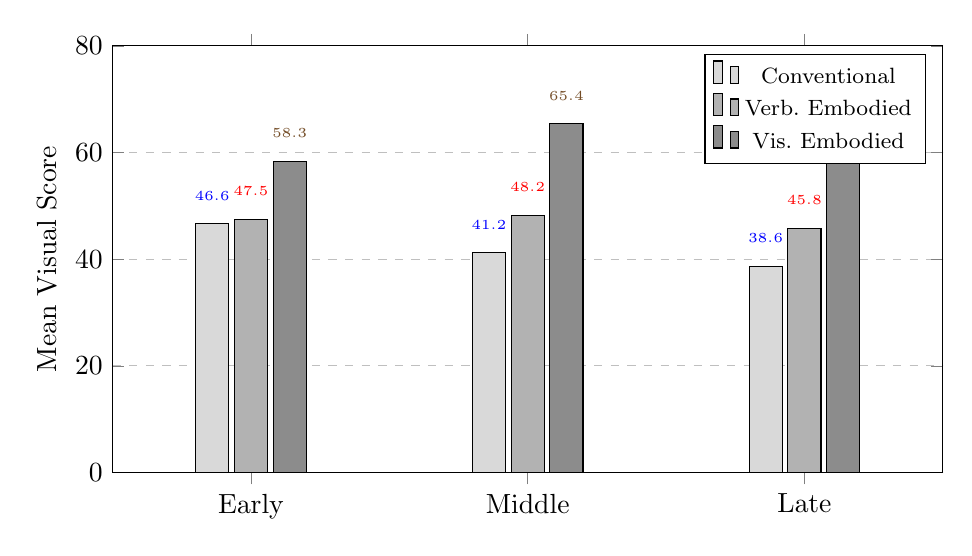
\begin{tikzpicture}
        \begin{axis}[
            ybar,
            bar width=12pt,
            width=\linewidth,
            height=7cm,
            symbolic x coords={Early,Middle,Late},
            xtick=data,
            ylabel={Mean Visual Score},
            ymin=0, ymax=80,
            enlarge x limits=0.25,
            legend style={at={(0.98,0.98)}, anchor=north east, font=\footnotesize},
            ymajorgrids=true,
            grid style=dashed,
            nodes near coords,
            nodes near coords style={font=\tiny\bfseries, yshift=5pt},
        ]
            \addplot+[fill=gray!30, draw=black] coordinates {(Early,46.6) (Middle,41.2) (Late,38.6)};
            \addplot+[fill=gray!60, draw=black] coordinates {(Early,47.5) (Middle,48.2) (Late,45.8)};
            \addplot+[fill=gray!90, draw=black] coordinates {(Early,58.3) (Middle,65.4) (Late,59.3)};
            \legend{Conventional, Verb.\ Embodied, Vis.\ Embodied}
        \end{axis}
    \end{tikzpicture}
    \caption{Mean visual engagement score by temporal position and subgroup. Conventional videos show a monotonic decline ($46.6 \to 38.6$), while visually embodied videos peak in the middle ($65.4$) and remain elevated throughout.}
    \label{fig:temporal}
\end{figure}

Figure~\ref{fig:temporal} reveals contrasting temporal patterns across subgroups. Conventional videos exhibit a monotonic decline in visual engagement from early (46.6) to late (38.6) segments, a drop of 8.0 points. Verbally embodied videos show a relatively flat trajectory (47.5, 48.2, 45.8), with a slight decline only in the final third. Visually embodied videos display an inverted-U pattern, peaking at 65.4 in the middle portion before returning to 59.3---still substantially higher than either other subgroup at any time point.

The decline in conventional video engagement likely reflects viewer fatigue with sustained lecture-format content. The stability of engagement in embodied videos suggests that physical demonstrations maintain viewer attention over longer durations. The mid-video peak in visually embodied videos may reflect that the core demonstration content typically occupies the middle portion, with introductory and concluding segments being less visually rich.


\subsection*{Instructional density and engagement}

We examined whether the instructional density rating (1--5 scale, as assessed by the video classification model) predicts visual engagement. As shown in Figure~\ref{fig:density}, visual correlation increases from 45.2\% at the lowest density level to 52.4\% at density levels 2 and 4, with level 3 slightly lower at 48.4\%.

\begin{figure}[ht]
    \centering
    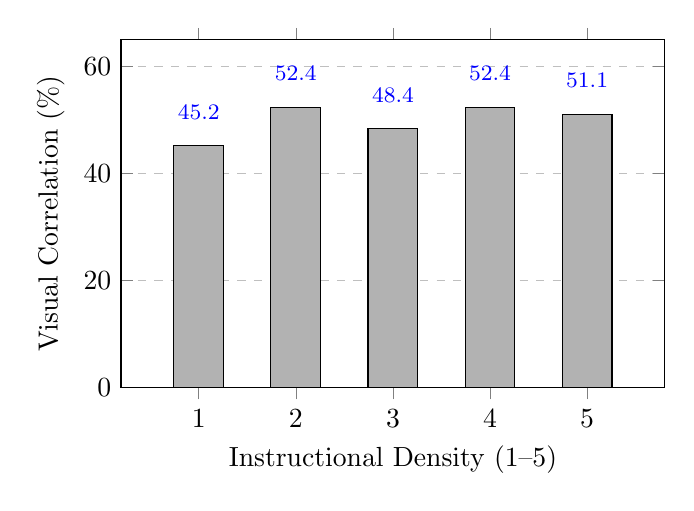
\begin{tikzpicture}
        \begin{axis}[
            ybar,
            bar width=18pt,
            width=0.7\linewidth,
            height=6cm,
            symbolic x coords={1,2,3,4,5},
            xtick=data,
            xlabel={Instructional Density (1--5)},
            ylabel={Visual Correlation (\%)},
            ymin=0, ymax=65,
            enlarge x limits=0.2,
            nodes near coords,
            nodes near coords style={font=\footnotesize\bfseries, yshift=6pt},
            ymajorgrids=true,
            grid style=dashed,
        ]
            \addplot+[fill=gray!60, draw=black] coordinates {
                (1,45.2)
                (2,52.4)
                (3,48.4)
                (4,52.4)
                (5,51.1)
            };
        \end{axis}
    \end{tikzpicture}
    \caption{Visual correlation by instructional density level. Low-density segments (level 1) show the weakest engagement, while levels 2--5 cluster around 48--52\%.}
    \label{fig:density}
\end{figure}

The overall trend indicates that low-density segments (level 1; $n = 1{,}169$) underperform relative to all other density levels, but the relationship is not strictly monotonic at higher levels. The lowest density segments---often transitions, pauses, or unfocused content---elicit the weakest visual engagement, while moderate-to-high density content generates comparable engagement regardless of whether it is rated 3, 4, or 5. The regression analysis confirms that instructional density does not significantly predict engagement after controlling for content type and hand visibility ($p = 0.106$).


\subsection*{Content profiles of high- and low-engagement videos}

To determine whether content composition explains video-level engagement differences, we compared the content type profiles of the top 25\% and bottom 25\% of videos ranked by visual correlation within each subgroup. Table~\ref{tab:top_bottom} presents the results for verbally embodied videos, where the contrast is most pronounced.

\begin{table}[ht]
    \centering
    \caption{Content type distribution (\%) for top- and bottom-quartile verbally embodied videos ranked by visual engagement. The largest difference is in hands-on demonstration content.}
    \label{tab:top_bottom}
    \begin{tabular}{lccc}
        \toprule
        Content Type & Top 25\% & Bottom 25\% & $\Delta$ \\
        \midrule
        Hands-on demo & \textbf{40.4} & 12.9 & +27.5 \\
        Equipment closeup & 12.1 & 9.2 & +2.9 \\
        Presenter talking & 13.7 & 13.5 & +0.2 \\
        Slide/PowerPoint & 8.5 & 8.9 & $-0.4$ \\
        Diagram/whiteboard & 6.4 & 7.9 & $-1.5$ \\
        Screen/software & 11.5 & \textbf{33.2} & $-21.7$ \\
        Animation/graphic & 1.6 & 2.3 & $-0.7$ \\
        Device in operation & 5.4 & 10.4 & $-4.9$ \\
        Other & 0.4 & 1.8 & $-1.4$ \\
        \bottomrule
    \end{tabular}
\end{table}

Among verbally embodied videos, the top-quartile engaged videos dedicate 40.4\% of their segments to hands-on demonstrations, compared to only 12.9\% in the bottom quartile---a difference of 27.5 percentage points. Conversely, the bottom-quartile videos contain 33.2\% screen/software content versus 11.5\% in the top quartile. This pattern demonstrates that within a single instructional modality, the proportion of hands-on content is a strong predictor of overall video engagement.

For conventional videos, the pattern is different: top-quartile conventional videos are dominated by diagram/whiteboard content (34.3\% vs.\ 22.4\% in the bottom quartile), while screen/software content is again associated with lower engagement (2.4\% in top vs.\ 9.9\% in bottom quartile). This suggests that the optimal content type varies by instructional modality---diagrams serve conventional instruction, while physical demonstrations serve embodied instruction---but in both cases, screen recordings consistently underperform.


\subsection*{Comparison with transcript-only analysis}

A key motivation for this study was the hypothesis that transcript-only analysis systematically underestimates the engagement of embodied instruction. Table~\ref{tab:paper_compare} presents the subgroup engagement rankings produced by the transcript-only analysis~\cite{zhang2025transcript} alongside the visual-channel rankings from the present study.

\begin{table}[ht]
    \centering
    \caption{Engagement ranking by subgroup under transcript-only versus visual-channel analysis. The metrics are not directly comparable (whole-video topic correlation vs.\ segment-level visual correlation), but the ranking reversal demonstrates the systematic bias of transcript-only approaches.}
    \label{tab:paper_compare}
    \begin{tabular}{lccc}
        \toprule
        & Conv. & Verb.\ Emb. & Vis.\ Emb. \\
        \midrule
        \multicolumn{4}{l}{\textit{Transcript-only analysis~\cite{zhang2025transcript}}} \\
        \quad Topic correlation (\%) & \textbf{61.2} & 51.3 & 11.2 \\
        \quad Ranking & 1st & 2nd & 3rd \\
        \addlinespace
        \multicolumn{4}{l}{\textit{Visual-channel analysis (this study)}} \\
        \quad Visual correlation (\%) & 52.3 & 54.3 & \textbf{68.2} \\
        \quad Ranking & 3rd & 2nd & 1st \\
        \bottomrule
    \end{tabular}
\end{table}

The ranking reversal is complete: visually embodied videos---which scored lowest under transcript-only analysis (11.2\%)---achieve the highest visual engagement (68.2\%). Conventional videos shift from first (61.2\%) to last (52.3\%). This reversal is not merely a reweighting; it reflects a fundamental change in which engagement channel is measured.

The transcript-only metric~\cite{zhang2025transcript} measures semantic correlation between viewer comments and video topics extracted from the full transcript at the whole-video level. For visually embodied videos (mean 13.6 WPM, 96 words per video), the transcripts contain negligible content, yielding near-zero correlation regardless of the videos' actual instructional quality. The visual-channel metric in the present study measures alignment between comments and frame-level captions, capturing the visual engagement that transcript analysis misses entirely.

These complementary analyses suggest that embodied and conventional videos achieve engagement through different channels: conventional instruction is strongest when measured through verbal content, while embodied instruction is strongest when measured through visual content. A complete evaluation of instructional video effectiveness requires both channels.


\subsection*{Summary of statistical tests}

Table~\ref{tab:stats} summarizes all statistical tests performed in this study.

\begin{table}[ht]
    \centering
    \caption{Summary of statistical tests. All tests use segment-level observations ($N = 9{,}997$) unless otherwise noted.}
    \label{tab:stats}
    \begin{tabular}{lrc}
        \toprule
        Test & Statistic & $p$-value \\
        \midrule
        \multicolumn{3}{l}{\textit{One-way ANOVAs}} \\
        \quad Visual corr.\ by content type & $F = 49.4$ & $< 10^{-79}$ \\
        \quad Transcript corr.\ by content type & $F = 23.2$ & $< 10^{-35}$ \\
        \quad Visual corr.\ by subgroup & $F = 99.4$ & $< 10^{-43}$ \\
        \quad Visual score by temporal bin & $F = 9.5$ & $< 10^{-4}$ \\
        \addlinespace
        \multicolumn{3}{l}{\textit{Two-way ANOVA}} \\
        \quad Content type main effect & $F = 39.5$ & $< 10^{-54}$ \\
        \quad Subgroup main effect & $F = 1.7$ & $0.191$ \\
        \quad Content $\times$ Subgroup interaction & $F = 8.4$ & $< 10^{-19}$ \\
        \addlinespace
        \multicolumn{3}{l}{\textit{Pairwise $t$-tests (visual)}} \\
        \quad Hands-on vs.\ slides & $t = 10.9$ & $< 10^{-27}$ \\
        \quad Hands-on vs.\ presenter & $t = 10.8$ & $< 10^{-26}$ \\
        \quad Hands-on vs.\ diagram & $t = 8.7$ & $< 10^{-18}$ \\
        \quad Device vs.\ presenter & $t = -3.2$ & $1.3 \times 10^{-3}$ \\
        \addlinespace
        \multicolumn{3}{l}{\textit{Other tests}} \\
        \quad Multiple regression ($R^2 = 0.050$) & $F = 40.2$ & $< 10^{-100}$ \\
        \quad Hands visible vs.\ not (visual) & --- & $< 10^{-40}$ \\
        \quad Narration absent vs.\ present & --- & $< 0.01$ \\
        \quad Video-level $r$ (verb.\ emb., $n=48$) & $r = 0.53$ & $1.2 \times 10^{-4}$ \\
        \quad Channel independence (overall) & $r = 0.14$ & $< 10^{-45}$ \\
        \bottomrule
    \end{tabular}
\end{table}


% ============================================================
% DISCUSSION
% ============================================================
\section*{Discussion}

This study provides the first segment-level, multimodal analysis of viewer engagement in robotics instructional videos, moving beyond group-level comparisons to identify the specific content features that drive learner interaction. Four principal findings emerge.

\textbf{Content type is the primary driver of engagement.} Hands-on demonstration segments achieve 64.1\% visual correlation---17.0 percentage points higher than slides and 28.5 points higher than screen recordings. The one-way ANOVA ($F = 49.4$, $p < 10^{-79}$) confirms that this is not attributable to chance, and the multiple regression identifies hands-on content ($\beta = +6.2$) and hand visibility ($\beta = +3.6$) as significant positive predictors, while screen content ($\beta = -13.2$) is the strongest negative predictor. These findings align with embodied cognition theory, which predicts that physical demonstrations activate sensorimotor processing that deepens engagement~\cite{barsalou2008grounded}.

\textbf{Content type fully mediates the subgroup effect.} The two-way ANOVA provides the most direct test of our central hypothesis. While the one-way ANOVA shows a large subgroup effect ($F = 99.4$, $p < 10^{-43}$), this effect disappears entirely when content type is controlled ($F = 1.7$, $p = 0.191$). This means that the subgroup label ``embodied'' or ``conventional'' carries no independent explanatory power; the engagement difference is entirely attributable to content composition. The significant interaction ($F = 8.4$, $p < 10^{-19}$) reflects the additional finding that embodied instructors produce higher-quality hands-on demonstrations (67.1--67.8\% vs.\ 43.9\% visual correlation for the same content type).

\textbf{The engagement advantage scales from segments to videos.} The video-level analysis confirms that the segment-level content type effect translates to overall video engagement. Among verbally embodied videos, the correlation between percentage of hands-on content and mean visual engagement is $r = 0.53$ ($p < 10^{-4}$). The top-quartile engaged verbally embodied videos contain 3.1 times more hands-on content than the bottom quartile (40.4\% vs.\ 12.9\%). These convergent results across multiple levels of analysis strengthen the causal interpretation: it is the hands-on content, not a confound, that drives engagement.

\textbf{Visual and verbal channels serve complementary engagement functions.} The weak overall correlation between visual and transcript scores ($r = 0.14$) demonstrates that the two channels operate largely independently. This independence is strongest for visually embodied videos ($r = 0.06$), which operate almost exclusively through the visual channel, and weakest for conventional videos ($r = 0.20$), where diagrams and verbal explanations are more tightly coupled. The complete ranking reversal between transcript-only and visual-channel analyses---conventional first vs.\ visually embodied first---further illustrates this complementarity. A comprehensive evaluation of instructional video effectiveness requires both channels; any single-channel metric will systematically favor the modality it measures.

The temporal analysis adds nuance: conventional video engagement declines monotonically from early to late segments ($46.6 \to 38.6$), suggesting viewer fatigue with sustained lecture content. Embodied video engagement remains stable or peaks mid-video, indicating that physical demonstrations sustain attention over longer durations. This temporal resilience represents a practical advantage of embodied instruction for longer-form content.

\textbf{Practical implications.} Instructors seeking to maximize visual engagement should prioritize hands-on demonstration content, ensure that physical manipulations are visually prominent (hands in frame), and minimize extended screen recording segments. The finding that screen/software content consistently ranks lowest across all analyses---lowest visual correlation, strongest negative regression coefficient, most prevalent in bottom-quartile videos---identifies a specific content type that should be used sparingly or interleaved with other formats. For conventional instruction where hands-on content is impractical, diagrams and whiteboard explanations provide the strongest visual engagement.

\textbf{Limitations.} The content classification was performed by a single large multimodal model (Gemini 2.0 Flash), and inter-rater reliability with human coders was not assessed. The correlation metrics depend on viewer comments that were elicited at the video level, then matched to individual segments, potentially introducing aggregation artifacts. The modest regression $R^2$ (0.050) indicates that content type and segment features explain only a fraction of the total variance in engagement; individual viewer differences, topic interest, and video production quality likely account for much of the unexplained variance. The audio-visual alignment score showed weak correlation with engagement ($r = 0.04$), which may reflect limitations in the alignment metric itself. Future work should incorporate human validation of content classifications, control for topic and production quality, and develop finer-grained measures of audio-visual synchrony.


% ============================================================
% METHODS
% ============================================================
\section*{Methods}

\subsection*{Dataset}

The dataset consists of 130 robotics instructional YouTube videos: 56 conventional and 74 embodied. Conventional videos feature lecture-style delivery through slides, diagrams, equations, and screen-recorded programming. Embodied videos present hands-on tutorials involving hardware assembly, wiring, calibration, and real-time robot operation. Videos span diverse robotics domains including robot arm assembly, mobile robot navigation, electronic circuit construction, computer vision, deep learning for robotics, combat robots, and drone systems. Video durations range from 92 to 5{,}760 seconds (median: 635 seconds), totaling approximately 26.5 hours of instructional content.

Based on analysis of speech rate distribution~\cite{zhang2025transcript}, the 74 embodied videos were subdivided into 48 verbally embodied ($\geq 60$ words per minute) and 26 visually embodied ($< 60$ WPM, silent demonstrations with minimal narration). This three-way classification---conventional ($n = 56$), verbally embodied ($n = 48$), and visually embodied ($n = 26$)---is maintained throughout all analyses.

\subsection*{Multimodal fusion pipeline}

The fusion analysis framework processes each video through a six-stage pipeline to produce segment-level engagement metrics for both visual and verbal channels. Figure~\ref{fig:pipeline} illustrates the complete data flow.

\begin{figure}[ht]
\centering
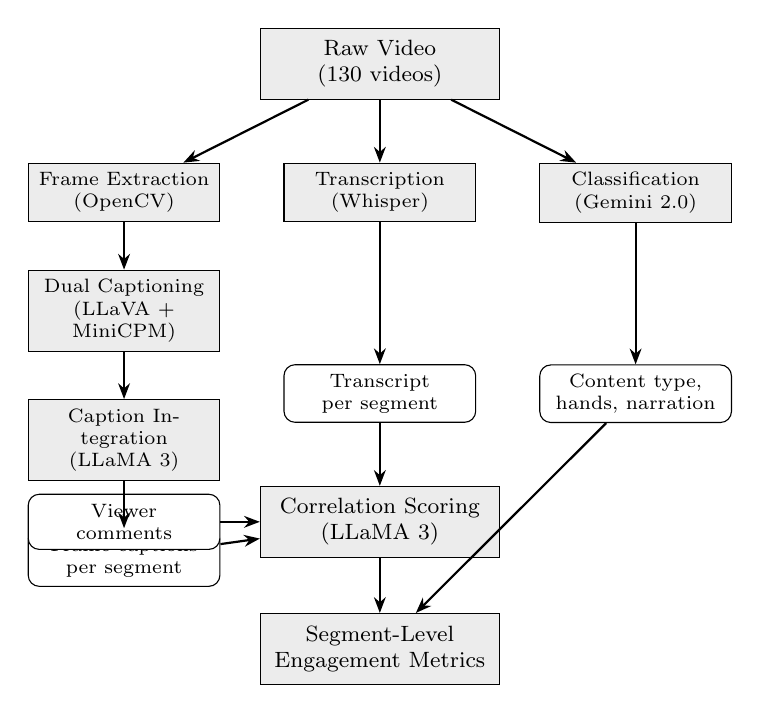
\begin{tikzpicture}[
    node distance=0.6cm and 0.8cm,
    block/.style={rectangle, draw, fill=gray!15, text width=2.8cm, minimum height=0.9cm, align=center, font=\footnotesize},
    smallblock/.style={rectangle, draw, fill=gray!15, text width=2.2cm, minimum height=0.7cm, align=center, font=\scriptsize},
    data/.style={rectangle, rounded corners, draw, fill=white, text width=2.2cm, minimum height=0.7cm, align=center, font=\scriptsize},
    arrow/.style={-{Stealth[length=2mm]}, thick},
]
    % Row 1: Input
    \node[block] (video) {Raw Video\\(130 videos)};

    % Row 2: Three parallel branches
    \node[smallblock, below left=0.8cm and 0.5cm of video] (frames) {Frame Extraction\\(OpenCV)};
    \node[smallblock, below=0.8cm of video] (whisper) {Transcription\\(Whisper)};
    \node[smallblock, below right=0.8cm and 0.5cm of video] (gemini) {Classification\\(Gemini 2.0)};

    % Row 3: Caption models
    \node[smallblock, below=0.6cm of frames] (caption) {Dual Captioning\\(LLaVA + MiniCPM)};

    % Row 3.5: Integration
    \node[smallblock, below=0.6cm of caption] (integrate) {Caption Integration\\(LLaMA 3)};

    % Row 4: Data outputs
    \node[data, below=0.6cm of integrate] (captions) {Frame captions\\per segment};
    \node[data, below=1.8cm of whisper] (transcript) {Transcript\\per segment};
    \node[data, below=1.8cm of gemini] (classify) {Content type,\\hands, narration};

    % Row 5: Correlation
    \node[block, below=0.8cm of transcript] (corr) {Correlation Scoring\\(LLaMA 3)};

    % Row 5 side: Comments
    \node[data, left=0.5cm of corr] (comments) {Viewer\\comments};

    % Row 6: Output
    \node[block, below=0.7cm of corr] (output) {Segment-Level\\Engagement Metrics};

    % Arrows
    \draw[arrow] (video) -- (frames);
    \draw[arrow] (video) -- (whisper);
    \draw[arrow] (video) -- (gemini);
    \draw[arrow] (frames) -- (caption);
    \draw[arrow] (caption) -- (integrate);
    \draw[arrow] (integrate) -- (captions);
    \draw[arrow] (whisper) -- (transcript);
    \draw[arrow] (gemini) -- (classify);
    \draw[arrow] (captions) -- (corr);
    \draw[arrow] (transcript) -- (corr);
    \draw[arrow] (comments) -- (corr);
    \draw[arrow] (corr) -- (output);
    \draw[arrow] (classify) -- (output);
\end{tikzpicture}
\caption{Multimodal fusion analysis pipeline. Raw videos are processed through three parallel branches: (1) frame extraction and dual-model captioning, (2) speech transcription, and (3) content classification. Visual captions and transcripts are independently correlated with viewer comments to produce dual-channel engagement metrics. Content classifications are joined with engagement scores for analysis.}
\label{fig:pipeline}
\end{figure}

\subsubsection*{Stage 1: Frame extraction.}
Frames are extracted from each video using OpenCV at a rate of one frame per 100 video frames (approximately one frame every 3.3 seconds at 30~fps). Videos encoded in AV1 codec are automatically transcoded to H.264 prior to extraction. The extracted frames serve as input to the visual captioning pipeline.

\subsubsection*{Stage 2: Audio transcription.}
Audio is transcribed using OpenAI Whisper~\cite{radford2023robust} with the \texttt{turbo} model, producing timestamped segments with start and end times in seconds. The timestamped output enables precise alignment between transcript segments and 10-second video intervals.

\subsubsection*{Stage 3: Visual captioning.}
Each extracted frame is independently captioned by two vision-language models: LLaVA~\cite{liu2023visual} and MiniCPM~\cite{yao2024minicpm}, both served locally via Ollama. The captioning prompt instructs the model to describe visual content objectively, focusing on visible elements (devices, slides, diagrams, text, hand positions) without inferring topics or intentions. The two captions per frame are then integrated into a single comprehensive caption using LLaMA~3~\cite{touvron2023llama}, which resolves contradictions and removes redundancy while preserving all factual observations from both sources. This dual-captioning approach improves coverage: LLaVA tends to capture spatial relationships and scene composition, while MiniCPM provides finer detail on text and small objects.

\subsubsection*{Stage 4: Temporal alignment and segmentation.}
Integrated captions and transcript segments are aligned on a shared timeline. Each caption is assigned a timestamp based on its frame index and the video's framerate. The aligned stream is then divided into fixed 10-second intervals, with each interval receiving all captions and transcript segments whose timestamps fall within its time window. This produces a uniform segmentation across all videos, with each segment containing both a visual summary (concatenated frame captions) and a verbal summary (concatenated transcript text).

\subsubsection*{Stage 5: Dual-channel correlation scoring.}
For each segment, viewer comments are independently compared against the visual captions and the transcript excerpt using LLaMA~3 via Ollama. Two separate prompts are used:

\begin{itemize}
    \item \textbf{Visual correlation prompt:} Instructs the model to determine whether a viewer comment refers to the visual content shown in the segment's frame captions. The model returns a boolean correlation judgment and a confidence score (0--100).
    \item \textbf{Transcript correlation prompt:} Instructs the model to determine whether a viewer comment discusses the speech or topic conveyed in the segment's transcript. The model returns a boolean correlation judgment and a confidence score (0--100).
\end{itemize}

Viewer comments were collected from two sources: (1) YouTube public comments retrieved via the YouTube Data API, and (2) student reflective responses submitted after viewing the videos during scheduled lecture sessions~\cite{zhang2025transcript}. To manage computational cost, a pre-filtering step using sentence-transformer embeddings (\texttt{all-mpnet-base-v2}) selects the top 200 most semantically relevant comments per video before correlation scoring. Each selected comment is scored against every segment, producing a matrix of visual and transcript correlation scores per video.

\subsubsection*{Stage 6: Metric aggregation.}
Per-segment metrics are computed by aggregating across all comment--segment pairs: visual correlation percentage (fraction of pairs with positive visual correlation), mean visual score, transcript correlation percentage, and mean transcript score. These segment-level metrics form the basis for all statistical analyses.


\subsection*{Video content classification}

Independent of the fusion pipeline, each video was classified at the segment level using Gemini 2.0 Flash~\cite{geminiteam2024gemini2} with direct video understanding. Unlike the fusion pipeline, which processes extracted frames and transcripts, the classification pipeline uploads the raw video file to the Gemini File API. The model watches the actual video content and classifies each 10-second segment.

To maintain output reliability, videos are processed in 5-minute chunks (approximately 30 segments per chunk). The classification prompt specifies the exact number of segments expected per chunk to enforce one-to-one correspondence with the fusion analysis segments. For each segment, the model assigns:

\begin{enumerate}
    \item \textbf{Content type}: One of nine mutually exclusive categories---\emph{hands\_on\_demonstration}, \emph{equipment\_closeup}, \emph{presenter\_talking}, \emph{slide\_or\_powerpoint}, \emph{diagram\_or\_whiteboard}, \emph{screen\_or\_software}, \emph{animation\_or\_graphic}, \emph{device\_in\_operation}, or \emph{other}. These categories were designed to span the full range of content observed in robotics instructional videos while maintaining mutual exclusivity.
    \item \textbf{Alignment score} (0--100): Degree to which the audio narration matches the visual content being shown. A score of 100 indicates perfect alignment (e.g., describing exactly what is on screen); a score near 0 indicates a mismatch (e.g., narrating theory while showing equipment).
    \item \textbf{Narration present}: Boolean indicating whether the instructor is actively speaking during the segment.
    \item \textbf{Hands visible}: Boolean indicating whether the instructor's hands appear in the frame, operationalizing the degree of physical interaction.
    \item \textbf{Instructional density} (1--5): Rating of how much instructional content is conveyed in the segment, from minimal (1, e.g., pauses, transitions) to maximal (5, e.g., dense technical explanation with demonstration).
\end{enumerate}

The classification was run on the Pittsburgh Supercomputing Center's Bridges-2 system via SLURM batch processing. Resume logic saves progress after each chunk, enabling recovery from API timeouts. Retry logic (3 attempts with exponential backoff at 30/60/90 seconds) handles transient server errors. A total of 9{,}997 segments across 129 videos were successfully classified. One 96-minute video exceeded Gemini's 1-million-token context limit and was excluded.


\subsection*{Data integration}

The fusion pipeline (Stages 1--6) and the classification pipeline produce independent per-segment data that are joined on video identifier and segment index. The joined dataset contains 9{,}997 observations, each with visual and transcript engagement metrics from the fusion pipeline and content type, narration, hand visibility, alignment, and density ratings from the classification pipeline. Video-level metrics are computed by averaging segment-level scores within each video ($N = 128$ videos with complete data from both pipelines).


\subsection*{Statistical analysis}

All statistical tests were conducted at the segment level ($N = 9{,}997$) unless otherwise noted. One-way ANOVA was used to test for differences in visual and transcript correlation across content types (9 levels), subgroups (3 levels), and temporal bins (3 levels). A two-way ANOVA with content type and subgroup as factors (including their interaction) was used to test whether the subgroup effect persists after controlling for content type; partial eta-squared ($\eta^2$) was computed as the effect size for each factor.

Independent-samples Welch's $t$-tests were used for pairwise comparisons between specific content types, with Cohen's $d$ reported as the effect size. Pearson correlation was computed between the alignment score and engagement metrics, between hands-on content proportion and video-level engagement, and between visual and transcript engagement scores (channel independence).

An ordinary least squares (OLS) multiple regression model was fit to predict visual engagement score from content type (dummy-coded, reference: slide/PowerPoint), hand visibility, narration, instructional density, and subgroup (dummy-coded, reference: conventional). This model estimates the independent contribution of each predictor while controlling for all others.

For the top/bottom quartile analysis, videos within each subgroup were ranked by mean visual correlation, and the content type distributions of the top and bottom 25\% were compared. Temporal analysis divided each video into three equal-length bins based on normalized segment position (0--0.33, 0.33--0.67, 0.67--1.0).

All $p$-values are reported without correction for multiple comparisons, as each test addresses a pre-specified hypothesis. Analyses were conducted using Python (scipy, statsmodels, pandas) on the Pittsburgh Supercomputing Center's Bridges-2 system.


% ============================================================
% REFERENCES
% ============================================================
\bibliography{sample}


\section*{Acknowledgements}

This work was funded by the National Science Foundation, Division of Engineering Education and Centers, Grant/Award Number: 2306285. Computational resources were provided by the Pittsburgh Supercomputing Center through the ACCESS allocation program.

\section*{Author contributions statement}

H.Z. conceived the study and supervised the research. B.L. developed the multimodal fusion framework, implemented the video classification pipeline, conducted all computational analyses, and drafted the manuscript. R.R. and N.G. contributed to data collection and video categorization. All authors reviewed the manuscript.

\section*{Additional information}

\textbf{Competing interests:} The authors declare no competing interests.

\end{document}
